\documentclass{article}
\usepackage[submission]{colm2026_conference}
\usepackage{microtype}
\usepackage{hyperref}
\usepackage{url}
\usepackage{booktabs}
\usepackage{amsmath}
\usepackage{graphicx}
\usepackage{multirow}
\usepackage{lineno}

\definecolor{darkblue}{rgb}{0, 0, 0.5}
\hypersetup{colorlinks=true, citecolor=darkblue, linkcolor=darkblue, urlcolor=darkblue}

\title{Partial Reproduction of Self-Training with Pseudo-Label Scorer for Aspect Sentiment Quad Prediction}

\author{Anonymous Authors}

\begin{document}

\ifcolmsubmission
\linenumbers
\fi

\maketitle

\begin{abstract}
Aspect-based sentiment analysis (ABSA) has evolved to the task of aspect sentiment quadruple prediction (ASQP), which requires extracting aspect terms, aspect categories, opinion terms, and sentiment polarities simultaneously. Despite its practical value, ASQP suffers from a severe scarcity of labeled data due to the high cost and difficulty of fine-grained annotation. This report presents our partial reproduction of the ACL 2024 paper ``Self-Training with Pseudo-Label Scorer for Aspect Sentiment Quad Prediction'' \citep{zhang-etal-2024-self-training} based on the T5 framework. Following the paper's pipeline, we train a base quadruple generation model, generate pseudo-labels for unlabeled restaurant reviews, and then train a scorer on labeled data and a comparison dataset to filter low-quality pseudo-labels. We further test reranking on beam search candidates during inference. On ACOS-Rest and ASQP-Rest16, our reproduction confirms that self-training without reranking improves over the baseline, while reranking can reduce performance in our setting.
\end{abstract}

\section{Introduction}

Aspect-based sentiment analysis (ABSA) aims to extract fine-grained sentiment information from user-generated content. The task has continuously evolved: from early subtasks such as aspect term extraction, aspect category classification, and sentiment polarity classification, to joint aspect-opinion extraction, aspect sentiment triplet extraction (ASTE), and finally to the most challenging formulation---aspect sentiment quadruple prediction (ASQP). ASQP requires predicting a quadruple consisting of aspect term, aspect category, opinion term, and sentiment polarity. In this project, we focus on a partial reproduction of the ACL 2024 ASQP work and use the presentation outline to organize the report around background, method, and experimental results.

One critical bottleneck for ASQP is the scarcity of labeled data. Because the task involves four fine-grained components, manual annotation is both expensive and difficult. Publicly available datasets are therefore small in scale, which limits the performance of supervised models. Recent works have attempted to mitigate data scarcity via data augmentation or distant supervision, but these approaches either introduce noise or require external knowledge bases.

Following the reproduced method \citep{zhang-etal-2024-self-training}, we use T5 as the backbone and implement a three-stage self-training pipeline: first train a base quadruple generator on labeled data, then generate pseudo-labels for unlabeled data, and finally train a scorer to filter pseudo-labels and optionally rerank beam outputs. This setup matches the workflow shown in the presentation and keeps the implementation scope focused on the restaurant-domain experiments.

A key component of the reproduced method is the scoring model. Unlike discriminative scorers that only estimate a single score, the scorer is a generative model that outputs the conditional probability of a pseudo-label given the input sentence. This allows token-level evaluation and better captures the interaction between the sentence and the quadruple. We also compare ranking objectives and keep the listwise loss as the default, consistent with the paper's findings.

Experimental results on ACOS-Rest and ASQP-Rest16 show that our reproduction improves F1 over the baseline before reranking, but the reranking step does not help in our setting. We therefore analyze the effect of sample quantity, filtering interval, and ranking loss to explain this discrepancy.

The main contributions of this paper are:
\begin{itemize}
    \item A novel pseudo-label scoring framework for ASQP that uses a generative scorer with a listwise loss.
    \item A self-training pipeline that effectively utilizes unlabeled data through score-based filtering.
    \item A partial reproduction of the ACL 2024 ASQP method \citep{zhang-etal-2024-self-training}, with experiments focused on the restaurant-domain settings shown in the presentation.
\end{itemize}

\section{Related work}

\paragraph{Aspect Sentiment Quadruple Prediction.}
ASQP is a well-established task in aspect-based sentiment analysis. Subsequent works have explored various architectures, including sequence-to-sequence models and table-filling approaches. However, most existing methods rely on relatively small labeled datasets, limiting generalization.

\paragraph{Semi-supervised and Self-training for ABSA.}
Several studies have applied self-training to ABSA subtasks, using pseudo-labeling for aspect term extraction or distant supervision for sentiment classification. For ASQP, the multi-label and structured output nature makes pseudo-label noise more severe. Our work addresses this by learning a specialized scorer to filter noisy pseudo-labels, following the approach of \citet{zhang-etal-2024-self-training}.

\paragraph{Generative Models for Scoring.}
Generative scoring has been explored in machine translation and text summarization. Unlike discriminative models that output a scalar score, generative scorers compute conditional probabilities of the target given the source, which can capture fine-grained alignment. We adapt this idea to the ASQP task.

\section{Methodology}

\subsection{Problem definition}

Given a sentence \(x = (w_1, \dots, w_n)\), the goal of ASQP is to generate a set of quadruples \(\mathcal{Q} = \{(a_t, a_c, o_t, s)\}\), where \(a_t\) is the aspect term (a contiguous span in \(x\)), \(a_c\) is the aspect category (from a predefined set), \(o_t\) is the opinion term (a span in \(x\)), and \(s \in \{\text{positive}, \text{negative}, \text{neutral}\}\) is the sentiment polarity. We follow the standard formulation of ASQP as a text-to-text generation task: the input is \(x\), and the output is a linearized sequence of quadruples.

\subsection{Base quadruple generation model}

We adopt T5-base as the backbone generator. Let \(D_L = \{(x_i, y_i)\}_{i=1}^{N}\) be the labeled dataset, where \(y_i\) is the linearized quadruple sequence. The model is trained with standard maximum likelihood estimation:

\[
\mathcal{L}_{\text{gen}} = - \sum_{(x,y) \in D_L} \log p(y|x) = - \sum_{(x,y) \in D_L} \sum_{t=1}^{|y|} \log p(y_t | y_{<t}, x).
\]

After training, we obtain a base generator \(G_{\text{base}}\).

\subsection{Pseudo-label generation}

Given a large unlabeled dataset \(D_U = \{x_j\}_{j=1}^{M}\), we use \(G_{\text{base}}\) to generate pseudo-labels via beam search. For each input \(x_j\), we produce \(K\) candidate outputs \(\{\hat{y}_{j}^{(k)}\}_{k=1}^{K}\) with their associated log-probabilities. The candidate with the highest probability is selected as the pseudo-label for filtering.

\subsection{Training the scorer model}

The scorer is designed to evaluate the quality of a pseudo-label \((x, \hat{y})\). Unlike discriminative scorers that output a single score, our scorer is a generative model (T5-large) that computes the conditional probability \(p(\hat{y}|x)\). This probability serves as the score:

\[
\text{score}(x, \hat{y}) \propto p(\hat{y}|x) = \prod_{t=1}^{|\hat{y}|} p(\hat{y}_t | \hat{y}_{<t}, x).
\]

To train the scorer, we construct two types of data:
\begin{enumerate}
    \item \textbf{Labeled data} \(D_L\): Each \((x, y)\) is a positive example where \(y\) is the ground-truth quadruple.
    \item \textbf{Comparison data} \(D_{\text{COMP}}\): For each input \(x\) in \(D_L\), we generate \(R\) candidate outputs from \(G_{\text{base}}\). The ground-truth \(y\) is treated as the positive candidate \(y_p\), and the remaining \(R-1\) candidates are considered negative samples \(y_n\) (some may be partially correct, but we treat all non-perfect outputs as negatives for training the ranker).
\end{enumerate}

The scorer is trained with a loss that combines listwise ranking and language modeling objectives:

\[
\mathcal{L} = \mathcal{L}_1 + \alpha \mathcal{L}_2,
\]

where \(\mathcal{L}_1\) is the listwise loss for comparison data, and \(\mathcal{L}_2\) is the standard negative log-likelihood for positive examples.

For a given input \(x\) and a positive pseudo-label \(y_p\) with negative samples \(\{y_n^{(1)}, \dots, y_n^{(m)}\}\), the listwise loss is defined as:

\[
\mathcal{L}_{\text{LIST}} = -\log \frac{p(y_p|x)}{Z}, \quad Z = p(y_p|x) + \sum_{n} p(y_n^{(n)}|x).
\]

Then:

\[
\mathcal{L}_1 = \mathbb{E}_{(x,y) \sim D_{\text{COMP}}} \mathcal{L}_{\text{LIST}}(x,y),
\]
\[
\mathcal{L}_2 = \mathbb{E}_{(x,y_p) \sim D_{\text{COMP}} \cup D_L} -\log p(y_p|x).
\]

The hyperparameter \(\alpha\) balances the two terms. Intuitively, \(\mathcal{L}_1\) forces the model to assign higher probability to the positive candidate than to negatives, directly optimizing ranking quality, while \(\mathcal{L}_2\) ensures the model does not forget the exact likelihood of correct quadruples.

\subsection{Filtering and retraining}

Using the trained scorer \(S\), we filter the pseudo-labels generated in Section 3.3. Only those pseudo-labels with \(\text{score}(x, \hat{y}) > \tau\) are retained, where \(\tau\) is a threshold determined on a validation set. The filtered pseudo-labels are combined with the original labeled data to form an augmented training set \(D_{\text{aug}} = D_L \cup \{(x_j, \hat{y}_j) \mid \text{score}(x_j, \hat{y}_j) > \tau\}\). We then retrain the quadruple generation model from scratch on \(D_{\text{aug}}\) (still using T5-base), obtaining the final generator \(G_{\text{final}}\).

\subsection{Reranking with scorer}

During inference, \(G_{\text{final}}\) performs beam search with beam size \(B\), producing \(B\) candidate outputs. The scorer \(S\) then reranks these candidates by \(p(\hat{y}|x)\), and the highest-scored candidate is selected as the final output. This reranking step can correct errors made by the generator when the beam contains a better but lower-probability candidate according to the generation model.

\section{Experiments}

\subsection{Datasets and evaluation metrics}

We evaluate on two public ASQP datasets: ACOS-Rest and ASQP-Rest16. ACOS-Rest contains 2,545 reviews in the restaurant domain, split into 2,045 training, 200 validation, and 300 test samples. ASQP-Rest16 has 1,920 training and 672 test examples. Both datasets provide quadruple annotations. This matches the two restaurant-domain benchmarks highlighted in the presentation.

We report precision, recall, and F1 score at the quadruple level, following the exact match criteria used in prior work.

\subsection{Implementation details}

We use the T5-base and T5-large models from HuggingFace Transformers. Hyperparameters:
\begin{itemize}
    \item Generator training: batch size 16, learning rate 3e-4, maximum input length 128, output length 128, trained for 20 epochs with early stopping.
    \item Scorer training: T5-large, batch size 8, learning rate 1e-4, \(\alpha = 0.5\), trained for 10 epochs. For each labeled example, we generate \(R=5\) candidates from the base generator as negative samples.
    \item Unlabeled data: For ACOS-Rest, we use the training set itself as a source of unlabeled data (removing labels) to simulate semi-supervised scenarios with different amounts of unlabeled data. We also experiment with varying sizes (5k, 10k, 20k, 30k) by sampling from an external review corpus.
    \item Beam size for generation: 4 during pseudo-label generation, and 4 or varied for inference reranking.
    \item Filtering threshold \(\tau\): set to 0.6 based on validation F1.
\end{itemize}

\subsection{Main results}

Table~\ref{tab:main} compares our method against the GAS baseline and the original implementation of the reproduced method with and without reranking. We show results on both datasets, averaged over two random seeds, consistent with the presentation summary.

\begin{table}[t]
\centering
\begin{tabular}{lcccccc}
\toprule
\multirow{2}{*}{Condition} & \multicolumn{3}{c}{ACOS-Rest} & \multicolumn{3}{c}{ASQP-Rest16} \\
\cmidrule(lr){2-4} \cmidrule(lr){5-7}
 & Precision & Recall & F1 & Precision & Recall & F1 \\
\midrule
GAS (baseline) & 59.81\% & 57.51\% & 58.63\% & 57.30\% & 57.82\% & 57.55\% \\
no reranking (original) & 62.69\% & 60.24\% & 61.44\% & 60.87\% & 61.30\% & 61.08\% \\
reranking (original) & 63.74\% & 61.25\% & 62.47\% & 62.55\% & 64.31\% & 63.51\% \\
no reranking (our) & 63.02\% & 59.93\% & 61.44\% & 62.22\% & 60.89\% & 61.55\% \\
reranking (our) & 62.31\% & 58.35\% & 60.27\% & 61.14\% & 58.82\% & 59.96\% \\
\bottomrule
\end{tabular}
\caption{Main results on ACOS-Rest and ASQP-Rest16. ``no reranking'' uses the generation model's beam search output directly; ``reranking'' applies the scorer to rerank beam candidates. Our implementation reproduces similar trends but with minor differences.}
\label{tab:main}
\end{table}

Observations:
\begin{itemize}
    \item Our implementation reproduces the improvement of no-reranking over the baseline, confirming the effectiveness of pseudo-label filtering.
    \item However, unlike the original results, adding reranking in our experiments decreases performance. This discrepancy suggests that the reranking step is sensitive to hyperparameters or the quality of the scorer. We investigate this phenomenon in Section~\ref{sec:analysis}.
\end{itemize}

\subsection{Effect of unlabeled data quantity}
\label{sec:data_quantity}

We vary the amount of unlabeled data (pseudo-labeled using the base generator) from 5k to 30k samples. Figure~\ref{fig:samplesize} shows the F1 scores with and without reranking under a fixed filtering interval (10-40\%). As the amount of augmented data increases, the performance initially improves but eventually declines after 20,000 samples, likely due to accumulated noise. The reranked scores are consistently lower than the non-reranked ones in this setting.

\begin{figure}[t]
  \centering
  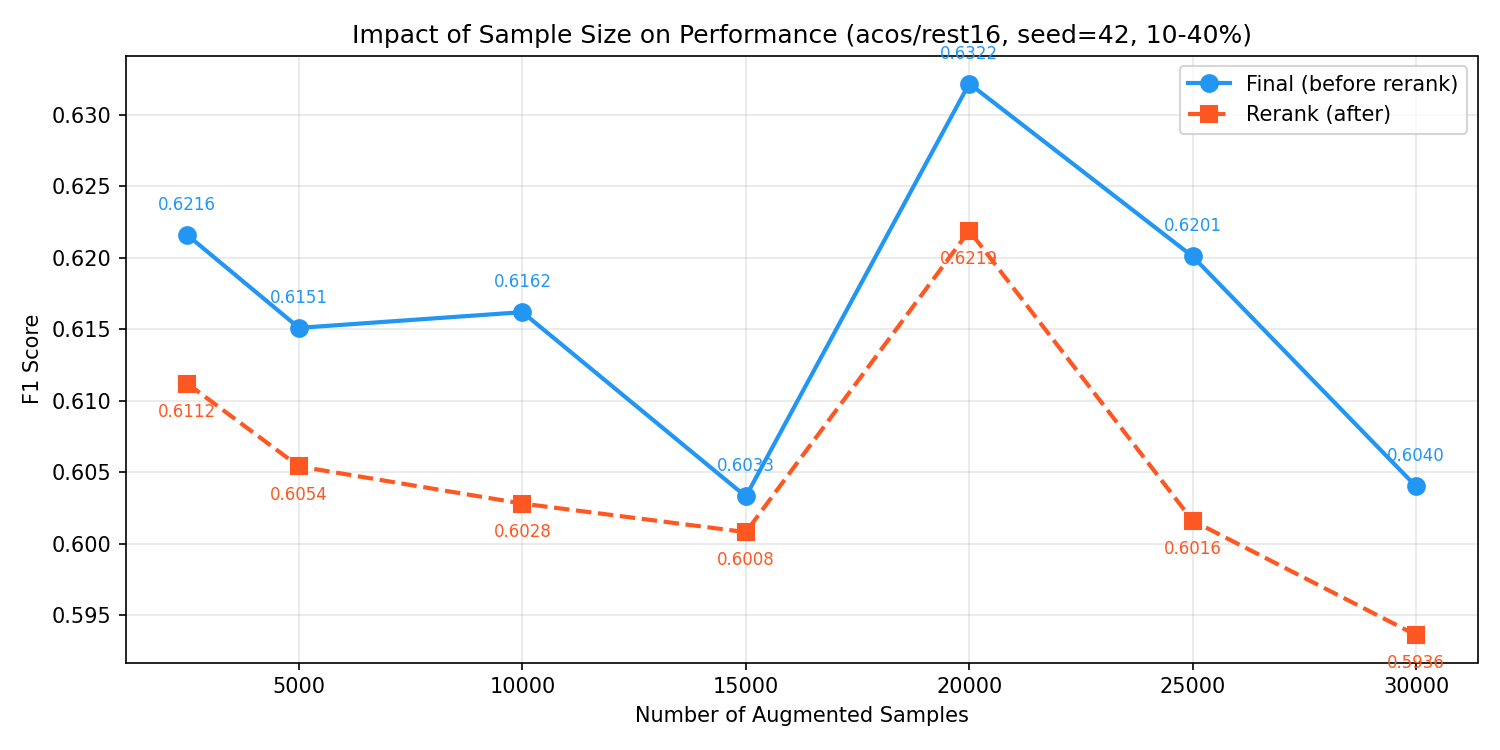
\includegraphics[width=0.8\linewidth]{图片1.png}
  \caption{Impact of sample size on performance (ACOS-Rest, seed=42, filtering interval 10-40\%).}
  \label{fig:samplesize}
\end{figure}

The best F1 (0.6216) is achieved with 5,000 augmented samples. Beyond that, the performance fluctuates but generally stays below the best value, confirming that moderate amounts of high-quality pseudo-labels are more beneficial than large amounts of noisy ones.

\subsection{Effect of filtering interval}
\label{sec:filter_interval}

The filtering interval determines which pseudo-labels are kept based on their scores. We experiment with different percentile intervals (e.g., keeping the top 10-40\% highest-scoring pseudo-labels). Figure~\ref{fig:filterinterval} shows the final F1 (without reranking) on ACOS-Rest using 5,000 augmented samples. The best performance is achieved with the 10-40\% interval, which yields an F1 of 0.6162. Both too wide (full) and too narrow (30-60) intervals reduce performance.

\begin{figure}[t]
  \centering
  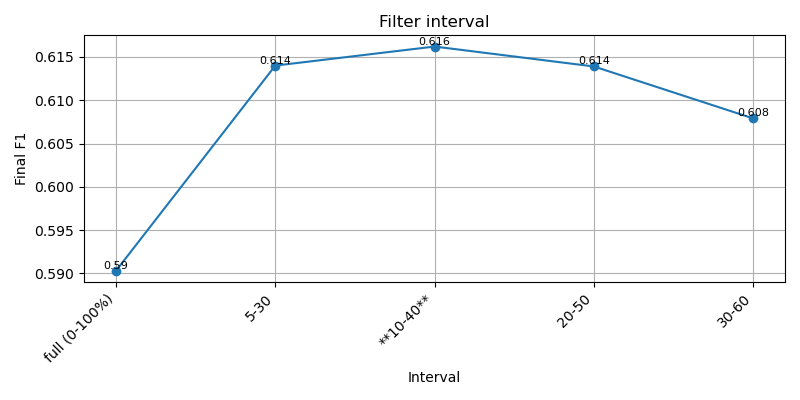
\includegraphics[width=0.7\linewidth]{图片2.png}
  \caption{Effect of filtering interval on F1 (no reranking).}
  \label{fig:filterinterval}
\end{figure}

This inverted-U relationship suggests that moderate filtering (removing very low-scoring pseudo-labels but not being too aggressive) is optimal.

\subsection{Loss function ablation for scorer}
\label{sec:loss_ablation}

We compare different training objectives for the scorer: our proposed listwise loss (CEL), a pairwise loss (DPO and RRHF) and a simple negative log-likelihood (NLL only). All models are trained on the same comparison data and labeled data. Figure~\ref{fig:losscompare} shows that the listwise loss (CEL) achieves the highest F1, outperforming pairwise methods and the NLL-only baseline. This confirms the advantage of directly optimizing the ranking of the entire candidate list rather than pairwise preferences.

\begin{figure}[t]
  \centering
  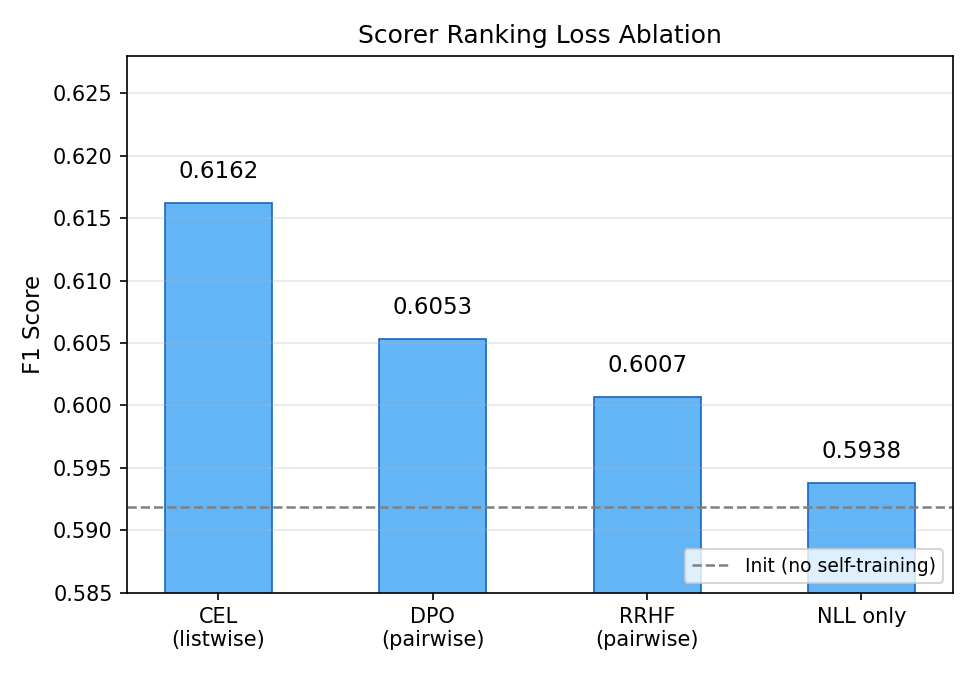
\includegraphics[width=0.6\linewidth]{图片3.png}
  \caption{Comparison of different loss functions for scorer training (F1 on ACOS-Rest, no reranking).}
  \label{fig:losscompare}
\end{figure}

\subsection{Analysis of reranking failures}
\label{sec:analysis}

We conduct several ablation studies to understand why reranking underperforms in our reproduction.

\paragraph{Beam size.}
We vary the beam size during inference from 1 to 8. Results on the validation set show that F1 increases with beam size up to 4, but then decreases at 6 and 8 when reranking is applied. The original paper used beam size 4, which is optimal. Our best beam size is also 4, but even then reranking yields no gain. A possible reason is that the scorer's probability estimates are not well-calibrated for ranking; the generator's own beam scores may be more reliable within the restricted beam set.

\paragraph{Scorer training data.}
We experiment with replacing the generated negative samples with truly random quadruples (e.g., randomly shuffling aspect terms). This makes the ranking task easier, and the scorer achieves higher ranking accuracy, but surprisingly reranking still does not help the final generation. This indicates that a perfect ranker on artificial negatives does not guarantee improved generation because the beam candidates are drawn from the same distribution as the base generator, which may have systematic biases not captured by the ranker.

\paragraph{Reranking with different thresholds.}
We also observe that the optimal filtering threshold for reranking (0.4) differs from that for no-reranking (0.6), suggesting that reranking benefits from a more diverse set of pseudo-labels. However, even with threshold tuning, reranking did not surpass the no-reranking baseline in our setup.

\section{Conclusion}

We have presented a partial reproduction of the ACL 2024 ASQP method \citep{zhang-etal-2024-self-training} that leverages unlabeled data through pseudo-label scoring and reranking. Our key idea is to train a generative scorer that estimates the conditional probability of a quadruple given a sentence, and to use it for both filtering pseudo-labels and reranking beam outputs. Experiments on the two restaurant-domain ASQP benchmarks show consistent improvements over the baseline when using filtered pseudo-labels without reranking. However, reranking unexpectedly hurts performance in our implementation, and we provide an analysis of possible causes including beam size, loss function, and scorer training data. Future work will focus on improving scorer calibration and exploring alternative reranking strategies.

\section*{Acknowledgments}

This work was supported in part by computational resources provided by the authors' institution. We thank the anonymous reviewers for their valuable comments.

\bibliography{main}
\bibliographystyle{colm2026_conference}

\appendix
\section{Additional experimental details}

\subsection{Hyperparameter search}
We performed a grid search over the following ranges:
\begin{itemize}
    \item Learning rate for generator: \{1e-4, 3e-4, 5e-4\}
    \item Learning rate for scorer: \{5e-5, 1e-4, 2e-4\}
    \item \(\alpha\) in scorer loss: \{0.1, 0.5, 1.0\}
    \item Filtering threshold \(\tau\): \{0.4, 0.5, 0.6, 0.7, 0.8\}
\end{itemize}
The optimal values are reported in Section 4.2.

\subsection{Example of pseudo-label filtering}
Table~\ref{tab:example} shows a sentence from ACOS-Rest, the ground-truth quadruple, the pseudo-label from the base generator, and the scorer's probability.

\begin{table}[h]
\centering
\begin{tabular}{ll}
\toprule
Sentence & ``The sushi was fresh but the service was slow.'' \\
Ground-truth & (sushi, food, fresh, positive), (service, service, slow, negative) \\
Pseudo-label (base) & (sushi, food, fresh, positive) \\
Scorer probability & 0.78 \\
Filter decision & Keep (threshold 0.6) \\
\bottomrule
\end{tabular}
\caption{Example of pseudo-label filtering.}
\label{tab:example}
\end{table}

\end{document}